% LaTeX path to the root directory of the current project
\providecommand{\econtexRoot}{}
\renewcommand{\econtexRoot}{..}
\providecommand{\econtexPaths}{LaTeX}\renewcommand{\econtexPaths}{\econtexRoot/LaTeX/econtexPaths}
\documentclass[\econtexRoot/BufferStockTheory]{subfiles}%% The \commands below are required to allow sharing of the same base code via Github between TeXLive on a local machine and Overleaf (which is a proxy for "a standard distribution of LaTeX").  This is an ugly solution to the requirement that custom LaTeX packages be accessible, and that Overleaf seems to ignore symbolic links (even if they are relative links to valid locations)
\providecommand{\econtex}{\econtexRoot/Resources/texmf-local/tex/latex/econtex}
\providecommand{\econtexSetup}{\econtexRoot/Resources/texmf-local/tex/latex/econtexSetup}
\providecommand{\econtexShortcuts}{\econtexRoot/Resources/texmf-local/tex/latex/econtexShortcuts}
\providecommand{\econtexBibMake}{\econtexRoot/Resources/texmf-local/tex/latex/econtexBibMake}
\providecommand{\econtexBibStyle}{\econtexRoot/Resources/texmf-local/bibtex/bst/econtex}
\providecommand{\econtexBib}{\econtexRoot/Resources/texmf-local/bibtex/bib/economics}
\providecommand{\notes}{\econtexRoot/Resources/texmf-local/tex/latex/handout}
\providecommand{\handoutSetup}{\econtexRoot/Resources/texmf-local/tex/latex/handoutSetup}
\providecommand{\handoutShortcuts}{\econtexRoot/Resources/texmf-local/tex/latex/handoutShortcuts}
\providecommand{\handoutBibMake}{\econtexRoot/Resources/texmf-local/tex/latex/handoutBibMake}
\providecommand{\handoutBibStyle}{\econtexRoot/Resources/texmf-local/bibtex/bst/handout}

\providecommand{\rootFromOut}{..} % Path back to root directory from output-directory

\providecommand{\EqDir}{\econtexRoot/Equations}
\providecommand{\FigDir}{\econtexRoot/Figures}
\providecommand{\CodeDir}{\econtexRoot/Code}
\providecommand{\DataDir}{\econtexRoot/Data}
\providecommand{\SlideDir}{\econtexRoot/Slides}
\providecommand{\TableDir}{\econtexRoot/Tables}
\providecommand{\ApndxDir}{\econtexRoot/Appendices}

\providecommand{\ResourcesDir}{\econtexRoot/Resources}
\ifnum\pdfshellescape=1
\providecommand{\LaTeXGenerated}{\econtexRoot/LaTeX} % Put generated files in subdirectory
\else
\providecommand{\LaTeXGenerated}{\econtexRoot/} % Put generated files in main directory (because not allowed in subdirectory)
\renewccommand{\EqDir}{\econtexRoot/Equations}
\fi
\providecommand{\econtexPaths}{\econtexRoot/Resources/econtexPaths}
\providecommand{\LaTeXInputs}{\econtexRoot/Resources/LaTeXInputs}

% LaTeX path to the root directory of the current project
\providecommand{\econtexRoot}{}
\renewcommand{\econtexRoot}{..}
\providecommand{\econtexPaths}{LaTeX}\renewcommand{\econtexPaths}{\econtexRoot/LaTeX/econtexPaths}
\input{\LaTeXFiles/econtex_onlyinsubfile}
%% LaTeX path to the root directory of the current project
\providecommand{\econtexRoot}{}
\renewcommand{\econtexRoot}{..}
\providecommand{\econtexPaths}{LaTeX}\renewcommand{\econtexPaths}{\econtexRoot/LaTeX/econtexPaths}
\documentclass{\econtex}
%\usepackage{\LaTeXFiles/BufferStockTheory}% Styling for whole paper (and subfiles)

%\input{\LaTeXFiles/econtex_onlyinsubfile}
%\onlyinsubfile{\externaldocument{BufferStockTheory}} % Get xrefs -- esp to appendix -- from main file; only works properly if main file has already been compiled; 
%\usepackage{tikz}

\begin{document}
  \hypertarget{RelatePFGICFHWCRICPFFVAC}{}

\begin{figure}[tbp]
  \centerline{
    \begin{tikzpicture}
      \node (thorn) {$\Pat$};
      \node (gamma) [right of = thorn] {$\PGro$};
      \node (rfree) [below of = thorn]{$\mathsf{\Rfree}$};
      \node (pffvacFac) [right of = rfree]{$\Rfree^{1/\CRRA}\PGro^{1 - 1/\CRRA} $}; % \left(\equiv (\Rfree \PGro)^{1/\CRRA}\PGro\right)
      \draw[->] (thorn) to node {$\mathrm{\PFGIC}$} (gamma);
      \draw[->] (thorn) to node [swap] {$\mathrm{\RIC}$} (rfree);
      \draw[->] (thorn) to node [swap] {$\mathrm{\PFFVAC}$} (pffvacFac);
      \draw[->] (gamma) to node {$\mathrm{\FHWC}$} (pffvacFac);
      \draw[->] (pffvacFac) to node {$\mathrm{\FHWC}$} (rfree);
    \end{tikzpicture}
  }
  \caption{Relation of \PFGIC, \FHWC, \RIC, and \PFFVAC} \label{fig:RelatePFGICFHWCRICPFFVAC}
  \footnotesize{Arrows reflect the direction of the relationship; an arrowhead points to the larger of the two quantities being compared.  For example, the topmost arrow, pointing from $\Pat$ to $\PGro$ indicates that $\PGro > \Pat$.}
\end{figure}

%\begin{figure}[h]
  \centerline{
    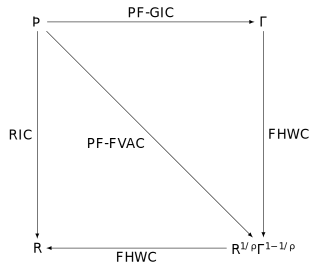
\includegraphics[width=3.5in]{\FigDir/RelatePFGICFHWCRICPFFVAC}
  }
  \caption{Relation of \PFGIC, \FHWC, \RIC, and \PFFVAC} \label{fig:RelatePFGICFHWCRICPFFVAC}
  \footnotesize{An arrowhead points to the larger of the two quantities being compared.  For example, the diagonal arrow indicates that $\Pat < \Rfree^{1/\CRRA}\PGro^{1-1/\CRRA}$, which is an alternative way of writing the {\PFFVAC}, \eqref{eq:PFFVAC}}
\end{figure}


\end{document}

% Delete up to four existing variants of BibTeX 

% Local Variables:
% eval: (setq TeX-command-list  (assq-delete-all (car (assoc "BibTeX" TeX-command-list)) TeX-command-list))
% eval: (setq TeX-command-list  (assq-delete-all (car (assoc "BibTeX" TeX-command-list)) TeX-command-list))
% eval: (setq TeX-command-list  (assq-delete-all (car (assoc "BibTeX" TeX-command-list)) TeX-command-list))
% eval: (setq TeX-command-list  (assq-delete-all (car (assoc "BibTeX" TeX-command-list)) TeX-command-list))
% eval: (setq TeX-command-list  (assq-delete-all (car (assoc "Biber"  TeX-command-list)) TeX-command-list))
% eval: (add-to-list 'TeX-command-list '("BibTeX" "bibtex LaTeX/%s" TeX-run-BibTeX nil t                                                                              :help "Run BibTeX") t)
% eval: (add-to-list 'TeX-command-list '("BibTeX" "bibtex LaTeX/%s" TeX-run-BibTeX nil (plain-tex-mode latex-mode doctex-mode ams-tex-mode texinfo-mode context-mode) :help "Run BibTeX") t)
% TeX-PDF-mode: t
% TeX-file-line-error: t
% TeX-debug-warnings: t
% LaTeX-command-style: (("" "%(PDF)%(latex) %(file-line-error) %(extraopts) -output-directory=LaTeX %S%(PDFout)"))
% TeX-source-correlate-mode: t
% TeX-parse-self: t
% eval: (cond ((string-equal system-type "darwin") (progn (setq TeX-view-program-list '(("Skim" "/Applications/Skim.app/Contents/SharedSupport/displayline -b %n LaTeX/%o %b"))))))
% TeX-parse-all-errors: t
% End:
